\section{Architecture (e.g., back-/frontend)}
This chapter describes the architecture of the application. 

\subsection{MVC Pattern}
This application is developed according to the MVC software architecture pattern. 
The MVC (Model-View-Controller) pattern, as depicted in the following diagram, is a software architectural pattern for implementing user interfaces. It divides an application into three interconnected components:

\begin{itemize}
    \item \textbf{Model:} Represents the data structure, business logic, and rules of the application. In your diagram, the model is represented by classes like FileModel, FolderModel, URLPair, and ConfigModel.
    \item \textbf{View:} Displays the data (the model) to the user and sends user commands to the controller. The ConsoleView is an example of this component in your diagram.
    \item \textbf{Controller:} Handles user input, interacts with the model, and selects the view to present. In the diagram, this is represented by CLIController.
    
\end{itemize}

The interaction between these components allows for efficient code separation, easier maintenance, and development. The Main class seems to act as the entry point of the application, orchestrating the MVC pattern. The diagram suggests that the Controller uses and updates the Model, and the View is also updated accordingly, maintaining a clear separation of concerns.

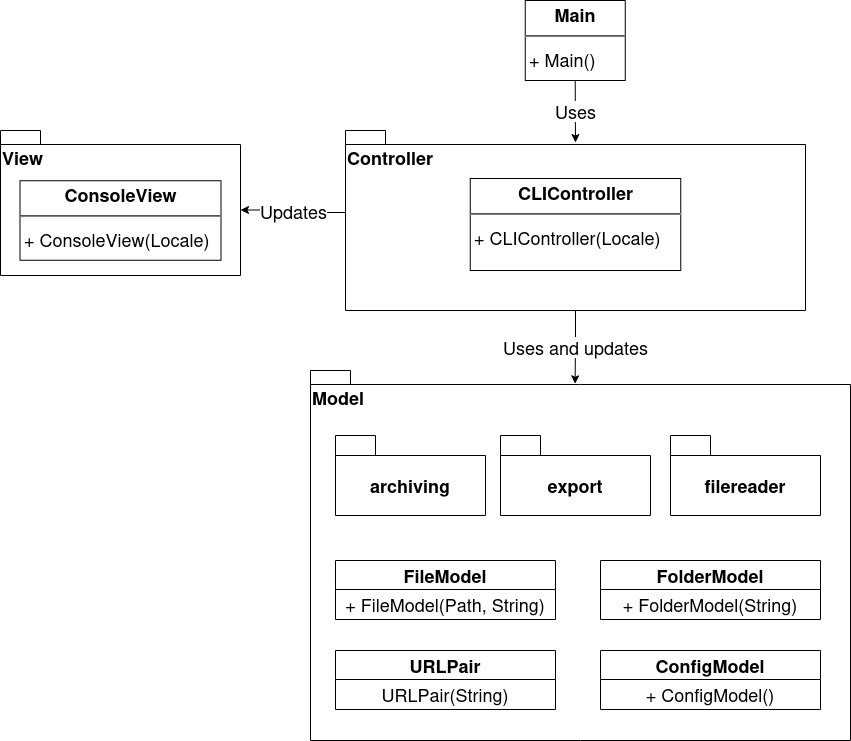
\includegraphics[width=1\textwidth]{diagrams/mvc_diagram-Highlevel_MVC.png}
\clearpage



